\documentclass[12pt,a4paper]{scrartcl}

\usepackage[english]{babel}
\usepackage[T1]{fontenc}
\usepackage{graphicx, subfig}
\usepackage[document]{ragged2e}
\usepackage{lmodern}
\usepackage{color}
\usepackage{amsmath}
\usepackage{graphicx}

% Für Verwendugn von Utnerstrichen ohne Escaping
\usepackage{underscore}

% Für Referenzen mit eigenem Text
\usepackage{hyperref}

% Für Codeblöcke
\usepackage{listings}

% Für Verwendung von Farben
\usepackage[usenames,dvipsnames,svgnames,table]{xcolor}

% Für Verktor-Pfeile
\usepackage{esvect}

% Für Größe der Seitenränder
\usepackage[margin=1in,footskip=0.5in]{geometry}

% Für Tabellen über Seiten hinweg
\usepackage{longtable}

% Für Header and Footer
\usepackage[automark]{scrpage2}

% Formatierung für Hyperref-Referenzen
\hypersetup{
	colorlinks,
	linkcolor={blue!50!black},
	citecolor={blue!50!black},
	urlcolor={blue!80!black}
}

% Generelle Formatierung für Code-Blöcke
\lstset{ %
	columns=fullflexible,
	keepspaces=true,
	frame=single,
	breaklines=true,
	breakautoindent=true,
	gobble=0,
	tabsize=2,
	belowskip=0pt
}

% Formatierung für Pseudo-Code
\lstdefinelanguage{PSEUDO} 
{ 
	xleftmargin=0pt, 
	xrightmargin=0pt,
	basicstyle=\small\ttfamily\color{Black},
	morekeywords={for, each, if, else},	
	keywordstyle = {\color{Orange}},
	sensitive=false,
	morecomment=[l]{//},
	morecomment=[s]{/*}{*/},
	morestring=[b]"
}

\title{Rendering and Manipulating Quad Meshes}
\author{Fabian Niehaus, Tuyet Nguyen}
\date{April 26, 2018}

\makeatletter

%% Generelle Kopf- und Fußzeilendefinition
\pagestyle{scrheadings}
\automark[section]{subsection} 
\clearscrheadfoot
\ihead[]{\@title}
\ohead[]{\rightmark}
\ifoot[]{\@author}

\begin{document}

\begin{titlepage}
	\centering
	\ \\[2cm]
	{\huge\textbf{\@title}} 
	\\[3cm]
	\large
	\textbf{Field of study:} Media informatics \\
	\textbf{Semester:} 4
	\\[2cm]
	\textbf{Date}: \@date
	\\[2cm]
	\textbf {Authors:}
	\\Fabian Niehaus
	\\501297
	\\Tuyet Nguyen
	\\5009445
\end{titlepage}

\newpage
%% Seitezahl auf 0 setzen
\setcounter{page}{0}
\tableofcontents

\newpage
%% Seitennummern einblenden
\ofoot[]{\pagemark}
\normalsize

\section{Abstract}
In this project we will build a C++ application that can read, render and write quad meshes as well as apply the Catmull-Clark subdivision algorithm. We will use QT Creator for programming, QT for window management and OpenGL for 3D rendering.

\section{Realisation}

\subsection{Creating an interface with QT}
First off, we create a new QT widget application. This allows us to use QT Creators design feature to set up our application's interface. A new QOpenGLWidget is placed and will be used as a placeholder for a new custom class inheriting QOpenGLWidgets functionality. This class, called OGLWidget, needs to implement the following methods: initializeGL (for setting up OpenGL), paintGL (for doing the actual rendering), resizeGL (for handling resizes of the display window). Additionally, the functions SetMaterialColor and InitLightingAndProjection\footnote{Taken from Prof. Dr. Martin Hering-Bertrams OpenGL_Example} are used.

\subsection{Creating the data structure}
In this step, the data structure for storing vertices and quads is implemented. This structure consist of a class "Vertex" containing the three coordinates and the valence and a class "Quad" containing the indices of four vertices, the indices of four adjacent quads, the index of its face vertex and the four indices of its edge vertices, the latter two being calculated in the process of the Catmull-Clark subdivision. The individual vertices and quads are stored in a vector list each.

\subsection{Reading the data from a file}
After creating the required data structure, a method for reading the vertices and faces from an .obj file is implemented. For this project we can assume that every face is a quad. The distinction between a vertex and a quad is made by the first letter in the line, a "v" for vertices and an "f" for quads. \\
Each line is read, and depending on the first letter a new Vertex or Quad is created and pushed to the respective vector.
If everything has been read correctly, a "true" value is returned.

\subsection{Rendering}
Depending on the desired way of rendering the object, different draw methods are implemented. These methods are then being called from the paintGL() function.

\subsubsection{Rendering as a wireframe}
At first, we want to render the object a wireframe without any specific lighting or normals. The method drawLines() implements this by going through the list of quads and connecting every two points that are next to each other, using GL_Lines. Every line needs two points as input, so every point is mentioned twice considering we need 4 lines per quad in total.

\subsubsection{Rendering as a cube}
After drawing the object as a wireframe we want to draw it as a solid cube with lighting. This is being achieved in the method drawQuads() which once again iterates over the list of quads. This time using GL_Quads, the four vertices of a quad are connected and the area inbetween is filled. The normal vector for this is calculated using the cross product of the two diagonals vectors.

\subsection{Calculation the vertex valence}
After making sure that the meshes are read and rendered correctly, the vertex valence is to be calculated. Vertex valence in this context means how many edges a single vertex is connected to. To calculate this, the following algorithm is used:


\begin{lstlisting}[language=PSEUDO]
for each verxtex 
	for each quad 
 		for each vertex of this quad
   			if index of both vertices is equal 
   				increase valence of vertex by 1
\end{lstlisting}

\subsection{Determining adjacent quads}
In order to determine each quads adjacent quads (or neighbors for short), we need to check if it has a shared edge with another quad. This is calculated by comparing if they share two vertices. The algorithm looks as follows:

\begin{lstlisting}[language=PSEUDO]
for each quad
	for i = 0 to 3 // since each quad has 4 vertices
		a = index of vertex at i
		b = index of vertex at (i+1)%4
		for each quad that is not the current one
			compare all vertices to a and b
			if a and b have a match
				add index of quad to current quads list of neighbors at index i 
\end{lstlisting} 

\subsection{Printing the data}
In order to verify the correctness of the results, all data is printed to the console. Additionally, each vertex (now with their valence) and quad (now with its neighbors) is written back to a .obj file.

\subsection{Catmull-Clark-Subdivision}

\subsubsection{Calculating the Face-Mask}
In the first step of the Catmull-Clark-Subdivision process, the so called Face-Mask is calculated. It describes the middle point of each quad. Mathematically speaking, it is the average of the four vertices of the quad:

$$ \vv{f} = \frac{1}{4}*( \vv{v}\textsubscript{0} + \vv{v}\textsubscript{1} + \vv{v}\textsubscript{2} + \vv{v}\textsubscript{3}) $$

This calculation is run for every quad. The resulting vertex is added to the list of vertices, and the index of it is stored within the quad.

\subsubsection{Calculating the Edge-Masks}
In the next step, the four edge masks are calculated. These vertices are the average between two end vertices of an edge and the face vertices of the two quads sharing this egde.\\
The formula for a single one of these points is:

$$ \vv{e} = \frac{1}{4} * (\vv{v}\textsubscript{a} + \vv{v}\textsubscript{b} + \vv{f} + \vv{f}\textsubscript{neighbor}) $$

This calculation is only run once per edge, meaning that only the quad with the lower index calculates the mask. The adjacent quad with the higher index only copies the reference. The following algorithm is used for the entire calculation.
\begin{lstlisting}[language=PSEUDO]
for each i = 0 to (size of quads - 1)
	Q = quad at index i
	for j = 0 to 4
		N = adjacent quad at index j in array of neigbors of Q
		if index of q is smaller than index of N
			calculate the edge mask using the formula explained above
		else
			for k = 0 to 4
				if value at index k of Ns adjacent quads = i
					add Ns edge mask of index k to Qs edge masks at index j		
\end{lstlisting} 

\subsubsection{Calculating the Vertex-Masks}
The last mask calculated is the Vertex-Mask. With this mask every original vertex of a quad is repositioned using the following formula:

$$ \vv{v}\textsubscript{new} = \frac{1}{(n\textsubscript{v})^{2}}*(2 \vv{e}\textsubscript{v\textsubscript{left}} + 2 \vv{e}\textsubscript{v\textsubscript{right}} - \vv{f}\textsubscript{v} +\vv{v} (n\textsubscript{v}(n\textsubscript{v}-3))) $$

The implementation is split into the three following steps:\\
\ \\
1.) Multiply every corner vertex with a product of its valence: $ \vv{v}\textsubscript{new} = \vv{v} (n\textsubscript{v}(n\textsubscript{v}-3)$
\begin{lstlisting}[language=PSEUDO]
for each vertex
	if vertex is corner vertex
		recalculate the vertex using the above formula
\end{lstlisting}
\ \\
\ \\
2.) Add edge vertices and subtract face vertex from each corner vertex of each quad: $\vv{v}\textsubscript{new} = \vv{v} + 2 \vv{e}\textsubscript{v\textsubscript{left}} + 2 \vv{e}\textsubscript{v\textsubscript{right}} - \vv{f}\textsubscript{v}$
\begin{lstlisting}[language=PSEUDO]
for each quad
	for each corner vertex of this quad
		recalculate the vertex using the above formula
\end{lstlisting}
\ \\
\ \\
3.) Divide each corner vertex by its valence squared: $ \vv{v}\textsubscript{new} = \vv{v} * \frac{1}{(n\textsubscript{v})^{2}}$
\begin{lstlisting}[language=PSEUDO]
for each vertex
	if vertex is corner vertex
		recalculate the vertex using the above formula
\end{lstlisting}

\subsubsection{Reconnecting the mesh}
In the final step of the Catmull-Clark-Subdivision every quad is divided into 4 smaller quads. These smaller quads are added to a newvector. After all quads have been subdivided, the original vector storing the quads is overwritten with the new vector storing four times the amout of quads.
\begin{lstlisting}[language=PSEUDO]
for each quad
	for j = 0 to 4
		v0 = corner vertex of the quad at index j
		v1 = edge vertex of the quad at index j
		v2 = face vertex of the quad
		v3 = edge vertex of the quad at index (j-1)%4 //tuned to always be positive
		create new quad with corner vertices v0 - v4 and store it
\end{lstlisting}

\section{Results}
\subsection{Number of vertices, faces (quads) and edges after subdivision}

\begin{tabular}{ll}
	Data used: cube.obj & Data used: threehole.obj \\
	\begin{tabular}{|l|l|l|l|}
		\hline
		Subdivisions & Vertices & Faces & Edges \\
		\hline
		0 & 8 & 6 & 12 \\
		\hline
		1 & 32 & 24 & 48 \\
		\hline
		2 & 128 & 96 & 192 \\
		\hline
		3 & 512 & 384 & 768 \\
		\hline
	\end{tabular}
	&
	\begin{tabular}{|l|l|l|l|}
		\hline
		Subdivisions & Vertices & Faces & Edges \\
		\hline
		0 & 64 & 68 & 136 \\
		\hline
		1 & 268 & 272 & 536 \\
		\hline
		2 & 1084 & 1088 & 2176 \\
		\hline
		3 & 4348 & 4348 & 8696 \\
		\hline
	\end{tabular}
	\\
\end{tabular}


\subsection{Rendering and subdivision}

\begin{longtable}{cc}
	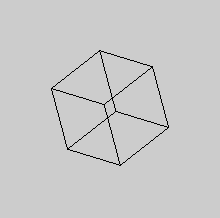
\includegraphics[width=150px, height=150px]{Images/cube-wireframe.png} 
	& 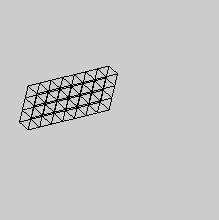
\includegraphics[width=150px, height=150px]{Images/threeholes-wireframe.png}  \\
	\multicolumn{2}{c}{Wireframe Cube and Threeholes} \\
	&\\
	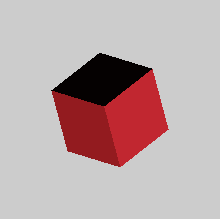
\includegraphics[width=150px, height=150px]{Images/cube-solid.png} 
	& 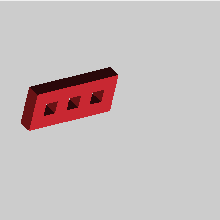
\includegraphics[width=150px, height=150px]{Images/threeholes-solid.png}  \\
	\multicolumn{2}{c}{Solid Cube and Threeholes} \\
	&\\
	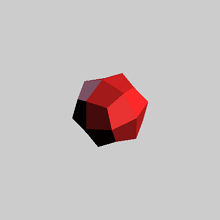
\includegraphics[width=150px, height=150px]{Images/cube-1sd.png} 
	& 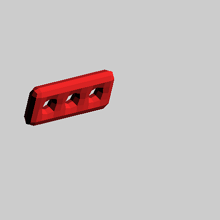
\includegraphics[width=150px, height=150px]{Images/threeholes-1sd.png}  \\
	\multicolumn{2}{c}{1 CC-Subdivision Cube and Threeholes} \\
	&\\
	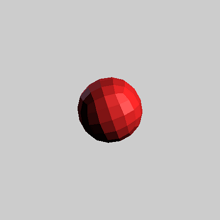
\includegraphics[width=150px, height=150px]{Images/cube-2sd.png} 
	& 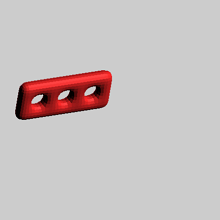
\includegraphics[width=150px, height=150px]{Images/threeholes-2sd.png}  \\
	\multicolumn{2}{c}{2 CC-Subdivisions Cube and Threeholes} \\
	&\\
	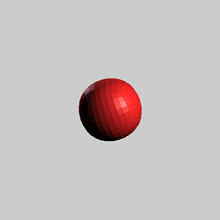
\includegraphics[width=150px, height=150px]{Images/cube-3sd.png} 
	& 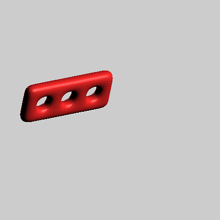
\includegraphics[width=150px, height=150px]{Images/threeholes-3sd.png}  \\
	\multicolumn{2}{c}{3 CC-Subdivisions Cube and Threeholes} \\
\end{longtable}

\section{Conclusion}
We were able to successfully build an application that can read and write any kind of boundary-free quad meshes, render them and perform Catmull-Clark-Subdivision on them. We gained a deeper understanding of how OpenGL and QT work and of the mathematics behing the specific subdivision concept. We will be able to extend the code for further applications and to reuse parts of it for other purposes e.g. calculation of Bezier surfaces.

\section{Acknowledgements}
\begin{itemize}
	\item User Martin B on StackOverflow for supplying the function for always positive modulos in C++
	\item The QT Company, GitHub, the developers of TeXStudio and the developers of MiKTEX for letting us use their software free of charge
	\item Any of the poor souls that had to discuss the maths and structure of this project with us
	\item Gut \& Guenstig Coffee for the long nights of debugging
\end{itemize}

\section{References}
\begin{itemize}
	\item Prof. Dr. Martin Hering-Bertram, Lecture CG18_1, HSB, 2018
\end{itemize}

\end{document}
